\documentclass{article}

\usepackage{physics} % Handy shortcuts like \pdv, \dd and much more
\usepackage{geometry} % smaller margins, can be adjusted if given arguments
\usepackage{siunitx} % the \si environment for units
\usepackage{mathtools} % The dcases environment, prettier than just cases
\usepackage{tikz} % For drawing picures
\usepackage{wrapfig} % Wrapping text around figures
\usepackage{cancel}

\title{Exercise 5 solutions - TFY4345 Classical Mechanics}
\date{2020}

\begin{document}
    \maketitle
    \section{Effective potential and scattering center}
        The total energy, as given by equation 4.14 in the compendium, is
        \begin{equation*}
            E = \frac{1}{2}m\left( \dot r^2 + (r\dot \theta)^2 \right) + V(r).
        \end{equation*}
        In a central potential, we have that $mr^2 \dot \theta = \ell$  is a conserved quantity, so we get 
        \begin{equation*}
            E = \frac{1}{2} m \dot r^2 + \left(\frac{\ell^2}{2 m r^2} + V(r) \right) = \frac{1}{2}m \dot r^2 + V_{\mathrm{eff}}(r).
        \end{equation*}
        This is an effective 1D problem, with an effective potential 
        \begin{equation*}
            V_{\mathrm{eff}}(r) = V(r) + \frac{\ell^2}{2 m r^2}
        \end{equation*}
        In order for the particle to reach the center, it need to have sufficiently high energy to overcome the potential barrier, i.e. $E > V_{\mathrm{eff}}(r \rightarrow 0)$. This can be written as
        \begin{equation*}
            E r^2 > r^2 V(r) + \frac{\ell^2}{2 m}, \quad r \rightarrow 0.
        \end{equation*}
        The l.h.s. goes to zero, so that the condition becomes 
        \begin{equation*}
            (r^2V(r))_{r \rightarrow 0} < - \frac{\ell^2}{2m}.
        \end{equation*}
        This can be fulfilled wither with $- k / r^2$, where $k > \ell^2 / 2m$, or if $V(r) = - A/r^n$, with $n > 2$ and $A$ a positive constant.

    \section{Scattering from a spherical obstacle}
        \begin{wrapfigure}{2}{0.32\textwidth}
            \vspace{-1cm}
            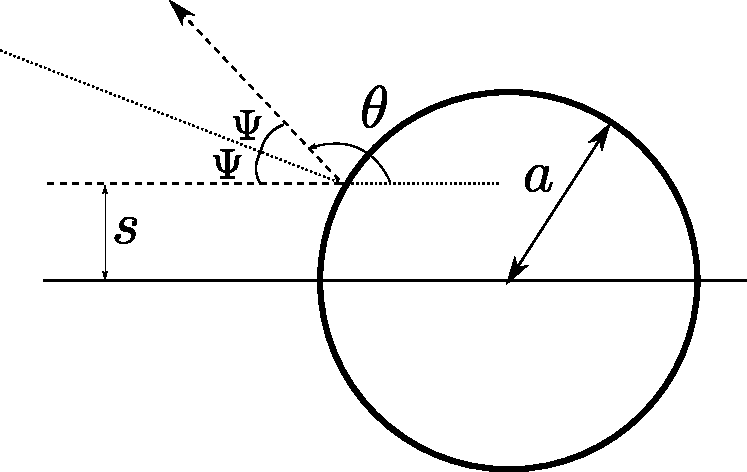
\includegraphics[width=0.32\textwidth]{figures/figure_2.pdf}
            \vspace{-2cm}
        \end{wrapfigure}
        The scattering angle $\theta$ satisfies $2 \Psi + \theta = \pi$. From the figure, we see that the impact parameter is given by $s = a \sin(\pi/2 - \theta /2 ) = a \cos(\theta / 2)$, so that 
        \begin{equation*}
            \left| \dv{s}{\theta} \right| = \frac{a}{2} \sin\left(\frac{\theta}{2}\right)
        \end{equation*}
        Using the formula for the differential cross section, as given in equation 4.40 in the compendium, we get
        \begin{equation*}
            \sigma(\theta) = \frac{s}{\sin(\theta)} \left| \dv{s}{\theta} \right| 
            = \frac{a^2}{2} \frac{\cos(\theta/2)\sin(\theta/2)}{\sin(\theta)}
             =\frac{a^2}{4}.
        \end{equation*}
        (b) The total cross section is therefore
        \begin{equation*}
            \sigma = 2 \pi \int_0^{\pi} \sigma(\theta) \sin(\theta) \dd \theta = \pi a^2.
        \end{equation*}
        This is physically sensible, since it is the actual cross-sectinoal area of the sphere.



    \section{Scattering by an attractive hard sphere}
        \begin{wrapfigure}{2}{0.3\textwidth}
            \vspace{-0.7cm}
            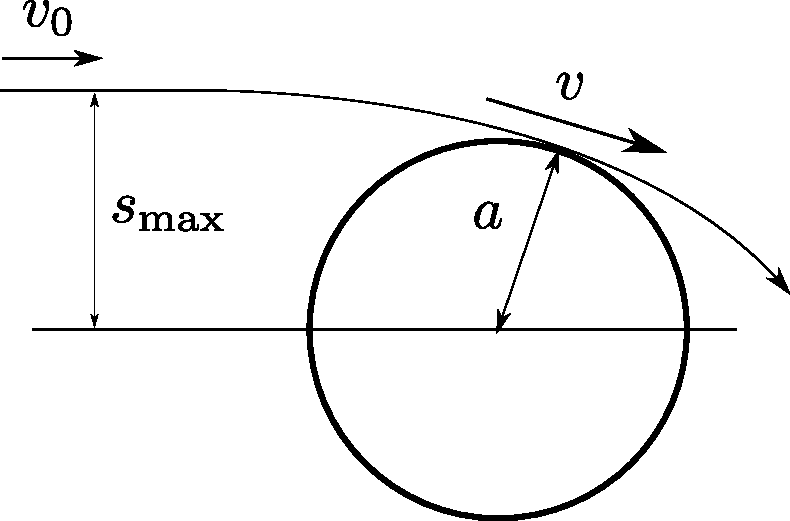
\includegraphics[width=0.3\textwidth]{figures/figure_3.pdf}
            \vspace{-1.3cm}
        \end{wrapfigure}
        The impact parameter $s_\mathrm{max}$ will send the particle just gracing the surface at $r=a$. Due to conservation of energy, we have that 
        \begin{equation*}
            E = \frac{1}{2} m v_0^2 = \frac{1}{2}mv^2 - \frac{k}{a}.
        \end{equation*}
        Furthermore, conservation of angular momentum means that $\ell$ infinitely far away is the same as when the particle touches the surface, so
        \begin{equation*}
            \ell = m v_0 s_\mathrm{max} = mva.
        \end{equation*}
        Combining thes two equations, we get
        \begin{equation*}
            s_\mathrm{max} = \frac{v}{v_0}a = a \sqrt{1 + \frac{2 k}{m a v_0^2}}.
        \end{equation*}
        All particles with impact parameter $s < s_\mathrm{max}$ will hit the surface, so that $\sigma_\mathrm{eff} = \pi s_\mathrm{max}^2$.


    \section{Average energies in the Kepler problem}
        (a) From the compendium, part 4E, we have 
        \begin{equation*}
            p = \frac{\ell^2}{m k}\, \quad \varepsilon^2 = 1 + \frac{2 E \ell^2}{m k^2}.
        \end{equation*}
        Eliminating $\ell$ gives us 
        \begin{equation*}
            E = - \frac{k}{2 p} \left(1 - \varepsilon^2\right).
        \end{equation*}
        The total energy is constant. This means that the average total energy also is constant:
        \begin{equation*}
            \expval{T} + \expval{V} = \expval{E} = E.
        \end{equation*}
        The viral theorem for a gravitational potential, example 12 in part 4D of the compendium, gives
        \begin{equation*}
            \expval{T} = - \frac{1}{2} \expval{V}.
        \end{equation*}
        Combining this gives
        \begin{align*}
            \expval{T} = \frac{k}{2 p} \left(1 - \varepsilon^2\right) \\
            \expval{V} = - \frac{k}{p} \left(1 - \varepsilon^2\right)
        \end{align*}
        (b) The solution to the Kepler problem in polar coordinates (found in the compendium) is 
        \begin{equation*}
            r = \frac{p}{1 + \varepsilon \cos(\theta)}.
        \end{equation*}
        The average potential energy over one period it
        \begin{equation*}
            \expval{V} = \frac{1}{t_p} \int_0^{t_p} \dd t V = -\frac{1}{t_p} \int_0^{t_p} \dd t \frac{k}{r}.
        \end{equation*}
        Combining these equations give
        \begin{align*}
            \expval{V} &= - \frac{1}{t_p}  \int_0^{t_p} \dd t \frac{k}{p} \left(1 + \varepsilon \cos(\theta)\right) = - \frac{k}{p t_p} \left(\int_0^{t_p} \dd t + \varepsilon \int_0^{t_p} \dd t\cos(\theta)\right) \\
            & = \frac{k}{p} \left(1 + \varepsilon\expval{\cos(\theta)}\right).
        \end{align*}
        We can find the the last integral by using $\ell = m r^2 \dot \theta$ and a change of variable
        \begin{align*}
            \expval{\cos(\theta)} & = \frac{1}{t_p}  \int_0^{t_p} \dd t \cos(\theta) 
            = \frac{1}{t_p}  \int_0^{2 \pi} \dd \theta \frac{1}{\dot \theta} \cos(\theta) = \frac{m }{\ell t_p} \int_0^{2 \pi} \dd \theta r(\theta)^2 \cos(\theta) \\
            &= \frac{m p^2}{\ell t_p} \int_0^{2 \pi} \dd \theta \frac{\cos(\theta) }{(1 + \varepsilon \cos(\theta))^2}.
        \end{align*}
        Using hint 2 and 3 we get
        \begin{align*}
            \expval{\cos(\theta)} & = \frac{m p^2}{\ell t_p} \int_0^{2 \pi} \dd \theta \frac{\cos(\theta) }{(1 + \varepsilon \cos(\theta))^2} 
            = - \frac{m p^2}{\ell t_p} \dv{\varepsilon} \int_0^{2\pi} \frac{\dd \theta}{1 + \varepsilon \cos(\theta)} \\
                & = - \frac{m p^2}{\ell t_p}\dv{\varepsilon} \frac{2 \pi}{\sqrt{1 - \varepsilon^2}} = - \frac{2 \pi m}{\ell t_p}  \frac{ p^2 \varepsilon}{(1 - \varepsilon^2)^{3/2}}.
        \end{align*}
        Then, using 
        \begin{equation*}
            t_p =  \frac{2 \pi m}{\ell^2} \frac{p^2}{(1 - \varepsilon^2)^{3/2}},
        \end{equation*}
        we get
        \begin{equation*}
            \expval{\cos(\theta)} = - \varepsilon,
        \end{equation*}
        so
        \begin{equation*}
            \expval{V} = \frac{k}{p}(1 - \varepsilon^2).
        \end{equation*}
        (c) Integrating the  kinetic energy by parts, with $\mathbf{\dot r}^2 = u' v$, gives 
        \begin{align*}
            \expval{T} & = \frac{m}{2 t_p}   \int_0^{t_p} \dd t \, \left(\dv{\mathbf{r}}{t}\right)^2 
            = \frac{m}{2 t_p} \left(\cancel{\mathbf{r} \cdot \dv{\mathbf{r}}{t}\bigg|_0^{t_p} } -   \int_0^{t_p} \dd t \, \mathbf{r} \cdot\dv[2]{\mathbf{r}}{t}\right)
        \end{align*}
        (as $\mathbf{r}(0) = \mathbf{r}(t_p)$, and $\mathbf{\dot r}(0) = \mathbf{\dot r}(t_p)$)
        \begin{align*}
            &  = - \frac{1}{2 t_p} \int_0^{t_p} \dd t \, \mathbf{r} \cdot \left(- \frac{k}{r^3} \mathbf{r}\right) = \frac{1}{2 t_p} \int_0^{t_p} \dd t \, \frac{k}{r} = - \frac{1}{2} \expval{V} = \frac{k}{2p}(1 - \varepsilon^2).
        \end{align*}
        This agrees with the result from the viral theorem.


\end{document}

